\chapter{Experimental Setup and Results}

In this chapter, I will describe our experimental setup and results. It includes a brief discussion of our optical tables setup (\ref{exp:laser-table} and \ref{exp:machine-table}), the implementation, optimization and performance of each steps (\ref{exp:mot}, \ref{exp:gm}, \ref{exp:pump}, \ref{exp:mt} and \ref{exp:odt}) and finally some basic characteristic of our BEC (\ref{exp:bec}).

\section{Laser System}\label{exp:laser-table}
The laser table is where we prepare all the light resonance with the Lithium-$7$ transition ($\approx671nm$). As discussed in the previous chapter, there are four distinct lines that we need in the experiment, the combination of $D1$, $D2$ with $F1$, $F2$. At a certain time, we need either $D1$ or $D2$ light with the probability of using both $F1$ and $F2$ at the same time and the laser table is designed to do just this.\\
\begin{figure}
  \begin{center}
    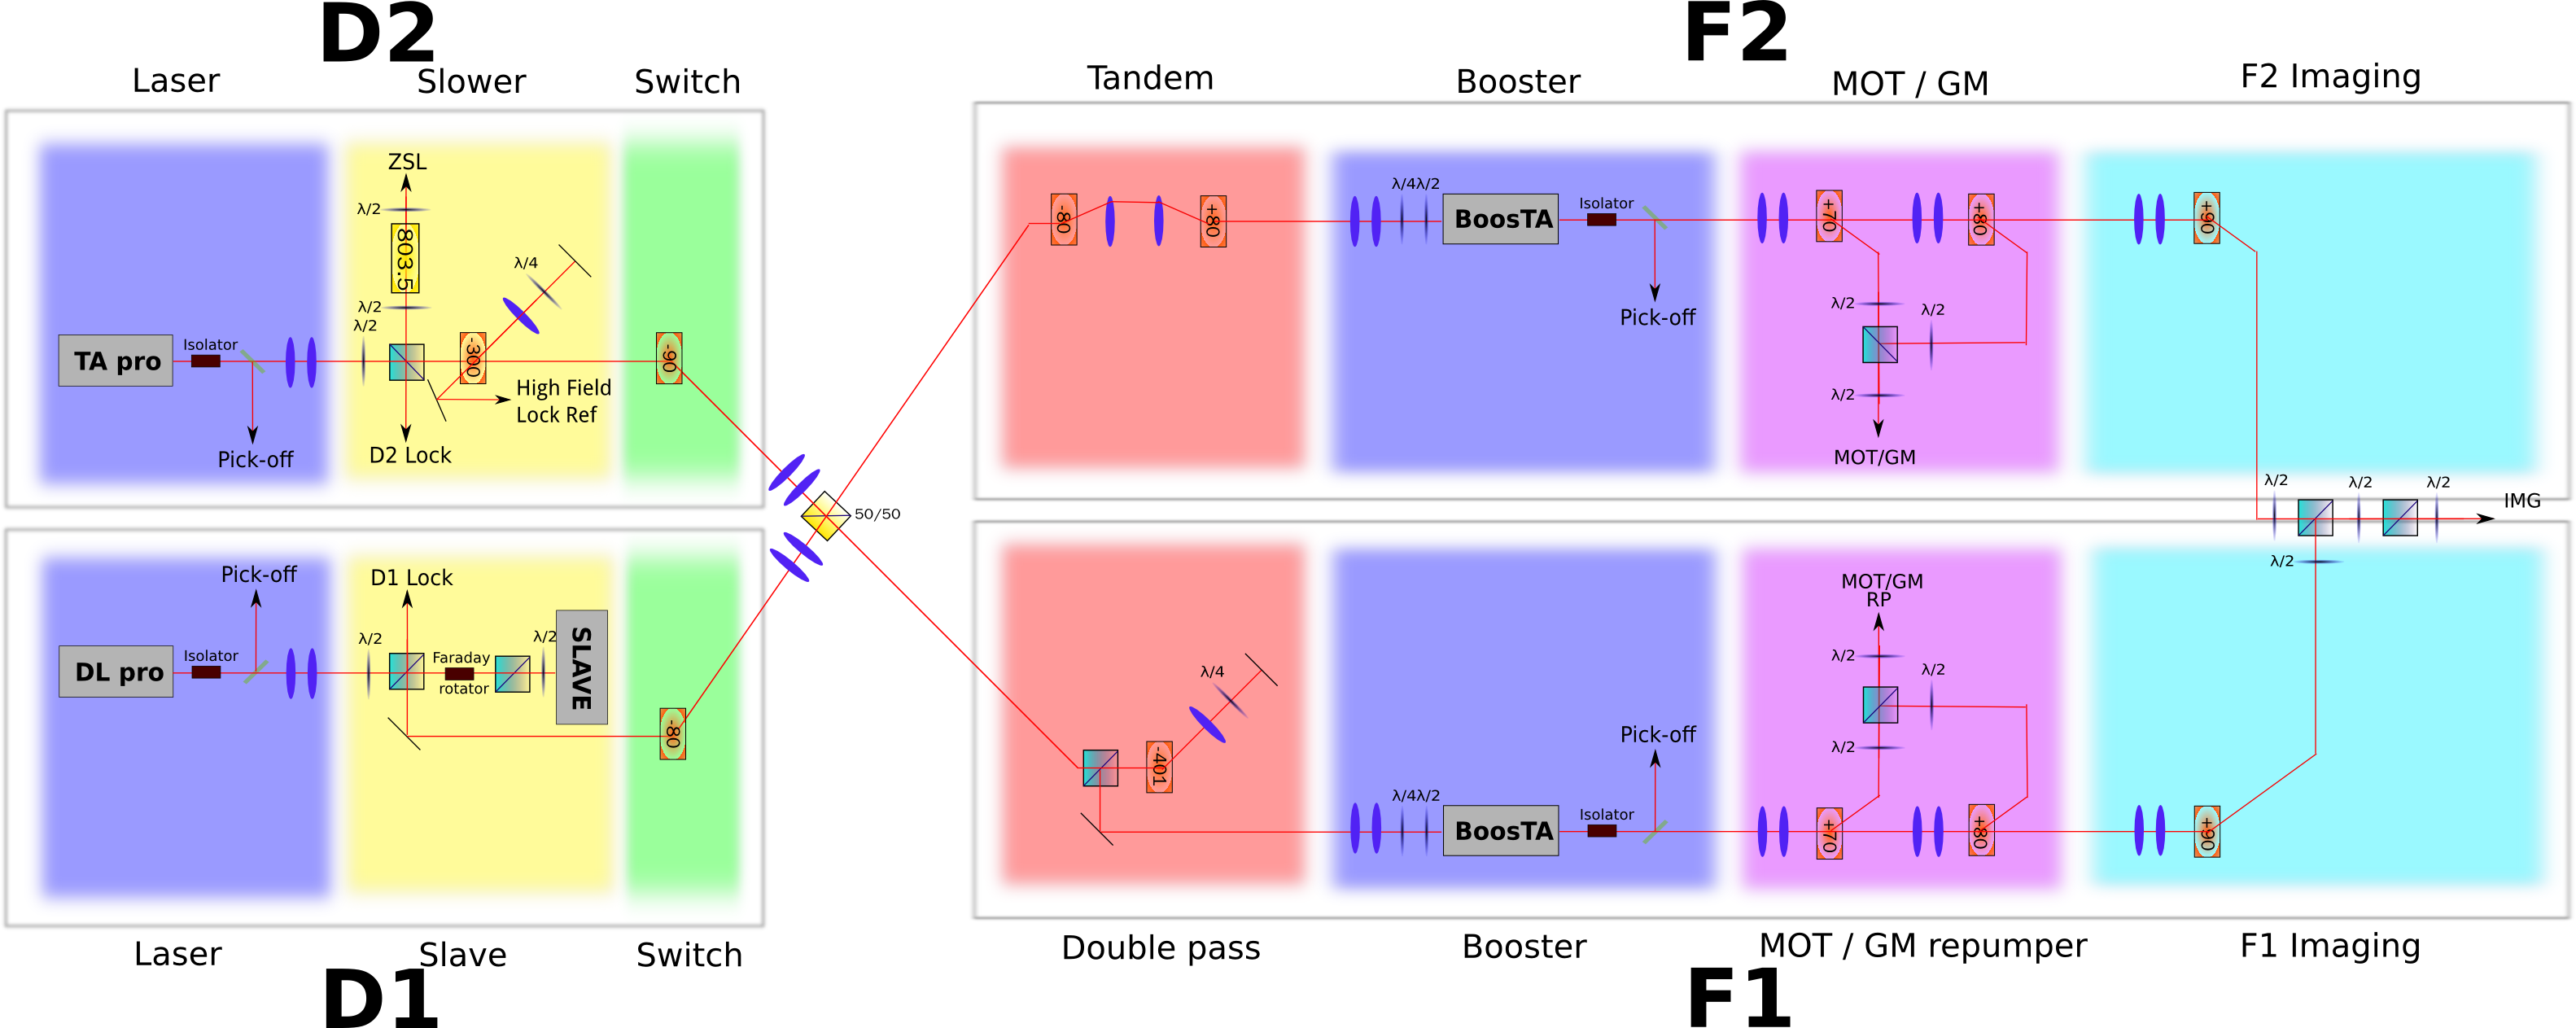
\includegraphics[width=14cm]{laser_table.png}
  \end{center}
  \caption{Schematic of the laser table design}
  \label{exp:laser-table-design}
\end{figure}\\
As shown in figure \ref{exp:laser-table-design}, since the separation between the $D1$ and $D2$ line ($\approx10GHz$) is larger than the range of common optical frequency shifters (e.g. AOMs), the $D1$ and $D2$ light are created separately using two diode lasers (TA pro and DL pro in figure \ref{exp:laser-table-design}). Both of these lasers are actively locked to the appropriate atomic transitions using saturated absorption spectroscopy to better than $2\text{MHz}$. For the $D2$ path, part of the light ($\approx80mW$) is red shifted and used as the Zeeman slower light ($ZSL$ in the figure) and the rest goes to the $D2$, $D1$ selecting switch, which uses two AOMs (acousto-optical modulator) and a $50$-$50$ cube to feed both the $F1$ and $F2$ path with either $D1$ and $D2$ light. For the $D1$ path, a slave diode is used to amplify the light before going to the switch.\\
\\
In the $F1$, $F2$ path, a tandem and a double pass are used to continuously shift the frequency of the laser (the double pass is also used to shift the light from $F2$ to $F1$). After that, the light in each path is amplified using tapered amplifier and then go through a polarization switch consists of two AOMs and a polarization beam splitter which can but the light into polarization maintaining fibers (MOT/GM and MOT/GM RP) with two orthogonal linear polarization's (the use of these beams is further described in section \ref{exp:mot-cage}). At the end of the chain, two more AOMs are used to control the light we put into the imaging fiber so that we can image on any of the four transitions. Each fibers also has a mechanical shutter that is used to block any possible leaking light that may cause heating.

\section{Vacuum Chamber and Main Coils Configuration}\label{exp:machine-table}

In this section, I am going to describe some important setup on the machine table where out vacuum chamber sits on.

\subsection{Optical Access of the Vacuum Chamber}\label{exp:chamber}
The windows and connections except the top and bottom window on our main vacuum chamber is shown in figure \ref{chamber-light}. There are in total $6$ MOT/Gray Molasses beams, $2$ ODT beams, $3$ Imaging beams, a plug and a Zeeman slower beam going into the chamber. When multiple colors need to be sent in through the same window, they are combined outside the vacuum chamber using appropriate dichroic.
\begin{figure}
  \begin{center}
    \begin{tikzpicture}[scale=0.8]
      % ODT windows
      \draw[rotate around={22.5:(0, 0)},line width=2] (-4.3, -.35) rectangle (4, .35);
      \draw[rotate around={-22.5:(0, 0)},line width=2] (-4.3, -.35) rectangle (4, .35);

      % MOT windows
      \draw[rotate around={45:(0, 0)},line width=2] (-3.2, -.7) rectangle (3.2, .7);
      \draw[rotate around={-45:(0, 0)},line width=2] (-3.2, -.7) rectangle (3.2, .7);

      % Slower windows
      \draw[line width=2] (0, -.8) rectangle (3.2, .8);
      \draw[line width=2] (-4, -.3) rectangle (0, .3);

      % Imaging windows
      \draw[line width=2] (-1.2, 0) rectangle (1.2, 3.2);
      \draw[line width=2] (-.4, 0) rectangle (.4, -3.2);

      % Main Chamber
      \draw[fill=white,line width=2] (0, 0) circle (3);

      % Coils
      \draw[line width=1,fill=brown] (0, 0) circle (2.5);
      \draw[line width=1] (0, 0) circle (2.3);
      \draw[line width=1] (0, 0) circle (2.1);
      \draw[line width=1] (0, 0) circle (1.9);
      \draw[line width=1] (0, 0) circle (1.7);
      \draw[line width=1,fill=white] (0, 0) circle (1.5);
      \path (0, 2) node[align=center,white] {\textbf{Main}\\\textbf{Coils}};

      % MOT beams
      \draw[line width=2,snake arrow,rotate around={45:(0, 0)},red] (6, 0) node[right] {MOT/GM} -- ++(-2.5, 0);
      \draw[line width=2,snake arrow,rotate around={-45:(0, 0)},red] (6, 0) node[right] {MOT/GM} -- ++(-2.5, 0);
      \draw[line width=2,snake arrow,rotate around={135:(0, 0)},red] (6, 0) node[right] {MOT/GM} -- ++(-2.5, 0);
      \draw[line width=2,snake arrow,rotate around={-135:(0, 0)},red] (6, 0) node[right] {MOT/GM} -- ++(-2.5, 0);

      % Imaging
      \draw[line width=1,snake arrow,rotate around={-90:(0, 0)},red] (6, 0) node[right,align=center] {Imaging/\\Dark State Pumping} -- ++(-2.5, 0);

      % ODT1
      \draw[line width=4,snake arrow,rotate around={22.5:(0, 0)}] (6, 0) node[right] {ODT} -- ++(-2, 0);
      \draw[line width=.5,snake arrow,rotate around={22.5:(0, 0)},red] (6, -0.2) -- ++(-2, 0);
      \path[rotate around={22.5:(0, 0)},red] (5, 0) node[below right,align=center] {Side\\Imaging};

      % ODT2
      \draw[line width=4,snake arrow,rotate around={-22.5:(0, 0)}] (6, 0) node[right] {ODT} -- ++(-2, 0);
      \draw[line width=.5,snake arrow,rotate around={-22.5:(0, 0)},red] (6, 0.2) -- ++(-2, 0);
      \path[rotate around={-22.5:(0, 0)},red] (5, 0) node[above right,align=center] {Side\\Imaging};
      \draw[line width=3,snake arrow,rotate around={-22.5:(0, 0)},green] (6, -0.3) -- ++(-2, 0);
      \path[rotate around={-22.5:(0, 0)},green] (5, -0.3) node[below left] {Plug};

      % Slower
      \draw[line width=2,snake arrow,red] (6, 0) node[right,align=center] {Zeeman\\Slower} -- ++(-2.5, 0);
      \draw[line width=4,->,rotate around={180:(0, 0)}] (6, 0) node[left,align=center] {Atoms\\From Oven} -- ++(-2, 0);
    \end{tikzpicture}
  \end{center}
  \caption{Top View of the Vacuum Chamber (Top/Bottom MOT/Gray Molasses beams not included, not to scale).}
  \label{chamber-light}
\end{figure}
\subsection{MOT-Gray Molasses Cage}\label{exp:mot-cage}
The delivery of the MOT and gray molasses beam from the two in-coupler on the laser table to the six output on the machine table is done with a polarization maintaining evanescent wave fiber splitter which takes the light from the two input fibers and split them equally into the six output fibers. However, the MOT beams and the gray molasses beams have different requirement in beam sizes. On one hand, the MOT needs a bigger beam size for a bigger capture volume. On the other hand, as discussed earlier, for the gray molasses to work effectively, high intensity, therefore smaller beam size, is required. In order to have a different size for the two beams coming out of the same fiber, we send in the two beams with orthogonal polarization's (figure \ref{exp:laser-table-design}) and add polarization dependent beam expenders after the fiber output to shape the two beams differently. This beam shaping is done with a cage system shown in figure \ref{mot-cage-design}. The upper beam path is used for expanding the MOT beam whereas the lower path shapes the gray molasses beam to a smaller size. Each of the four lenses can slide in the cage, which are used to tweak the size and divergence of the beams. The alignment between beams is done with the two bottom mirrors and the two half wave-plates between the two polarization beam splitter cubes are used to balance the intensities.
\begin{figure}
  \begin{center}
    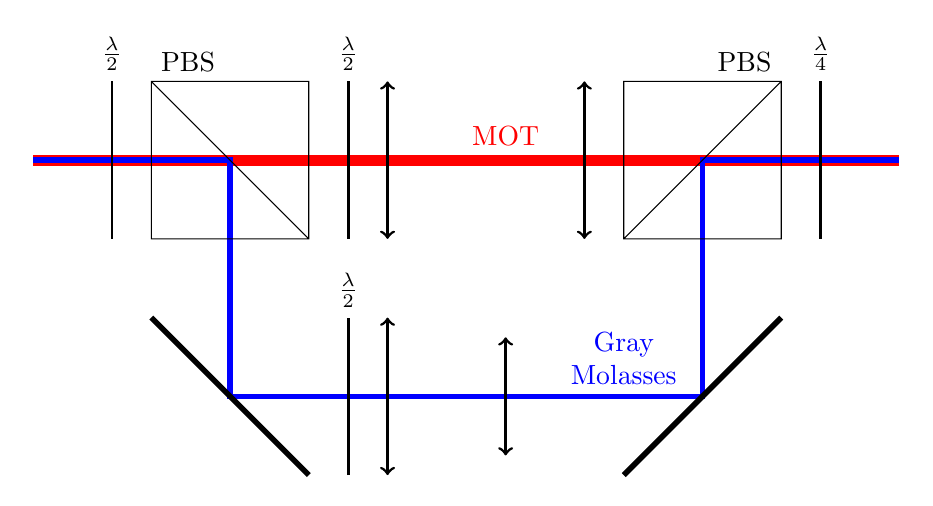
\begin{tikzpicture}
      \draw[line width=4,red] (-1, 1) -- (5, 1) node[above] {MOT} -- (10, 1);

      \draw[line width=2,blue] (-1, 1) -- (1.5, 1) -- ++(0, -3) -- (6.5, -2) node[above,align=center] {Gray\\Molasses} -- (7.5, -2) -- (7.5, 1) -- (10, 1);

      \draw[line width=1] (0, 0) -- ++(0, 2) node[above] {$\frac{\lambda}{2}$};
      \draw (0.5, 2) rectangle ++(2, -2) -- ++(-2, 2) node[above right] {PBS};
      \draw[line width=1] (3, 0) -- ++(0, 2) node[above] {$\frac{\lambda}{2}$};
      \draw[line width=1,<->] (3.5, 0) -- ++(0, 2);
      \draw[line width=1,<->] (6, 0) -- ++(0, 2);
      \draw (6.5, 0) rectangle ++(2, 2) node[above left] {PBS} -- ++(-2, -2);
      \draw[line width=1] (9, 0) -- ++(0, 2) node[above] {$\frac{\lambda}{4}$};

      \draw[line width=2] (2.5, -3) -- ++(-2, 2);
      \draw[line width=1] (3, -3) -- ++(0, 2) node[above] {$\frac{\lambda}{2}$};
      \draw[line width=1,<->] (3.5, -3) -- ++(0, 2);
      \draw[line width=1,<->] (5, -2.75) -- ++(0, 1.5);
      \draw[line width=2] (8.5, -1) -- ++(-2, -2);
    \end{tikzpicture}
  \end{center}
  \caption{MOT/Gray Molasses Cage.}
  \label{mot-cage-design}
\end{figure}

\subsection{Main Coils Configuration}\label{exp:coil}
In our experiment, a lot of different field configurations are used for different purpose. All of these configurations have to be implemented using our main coil which has five independent layers closed to the Helmholtz condition on each sides with sub millisecond switching time between them. A modified H-bridge (figure \ref{exp:coil-control}) was build with IGBTs in order to accomplish these goals using the minimum amount of independent layers, IGBTs and power supplies. The list of possible configurations are shown in table \ref{exp:coil-config}.
\begin{figure}
  \begin{center}
    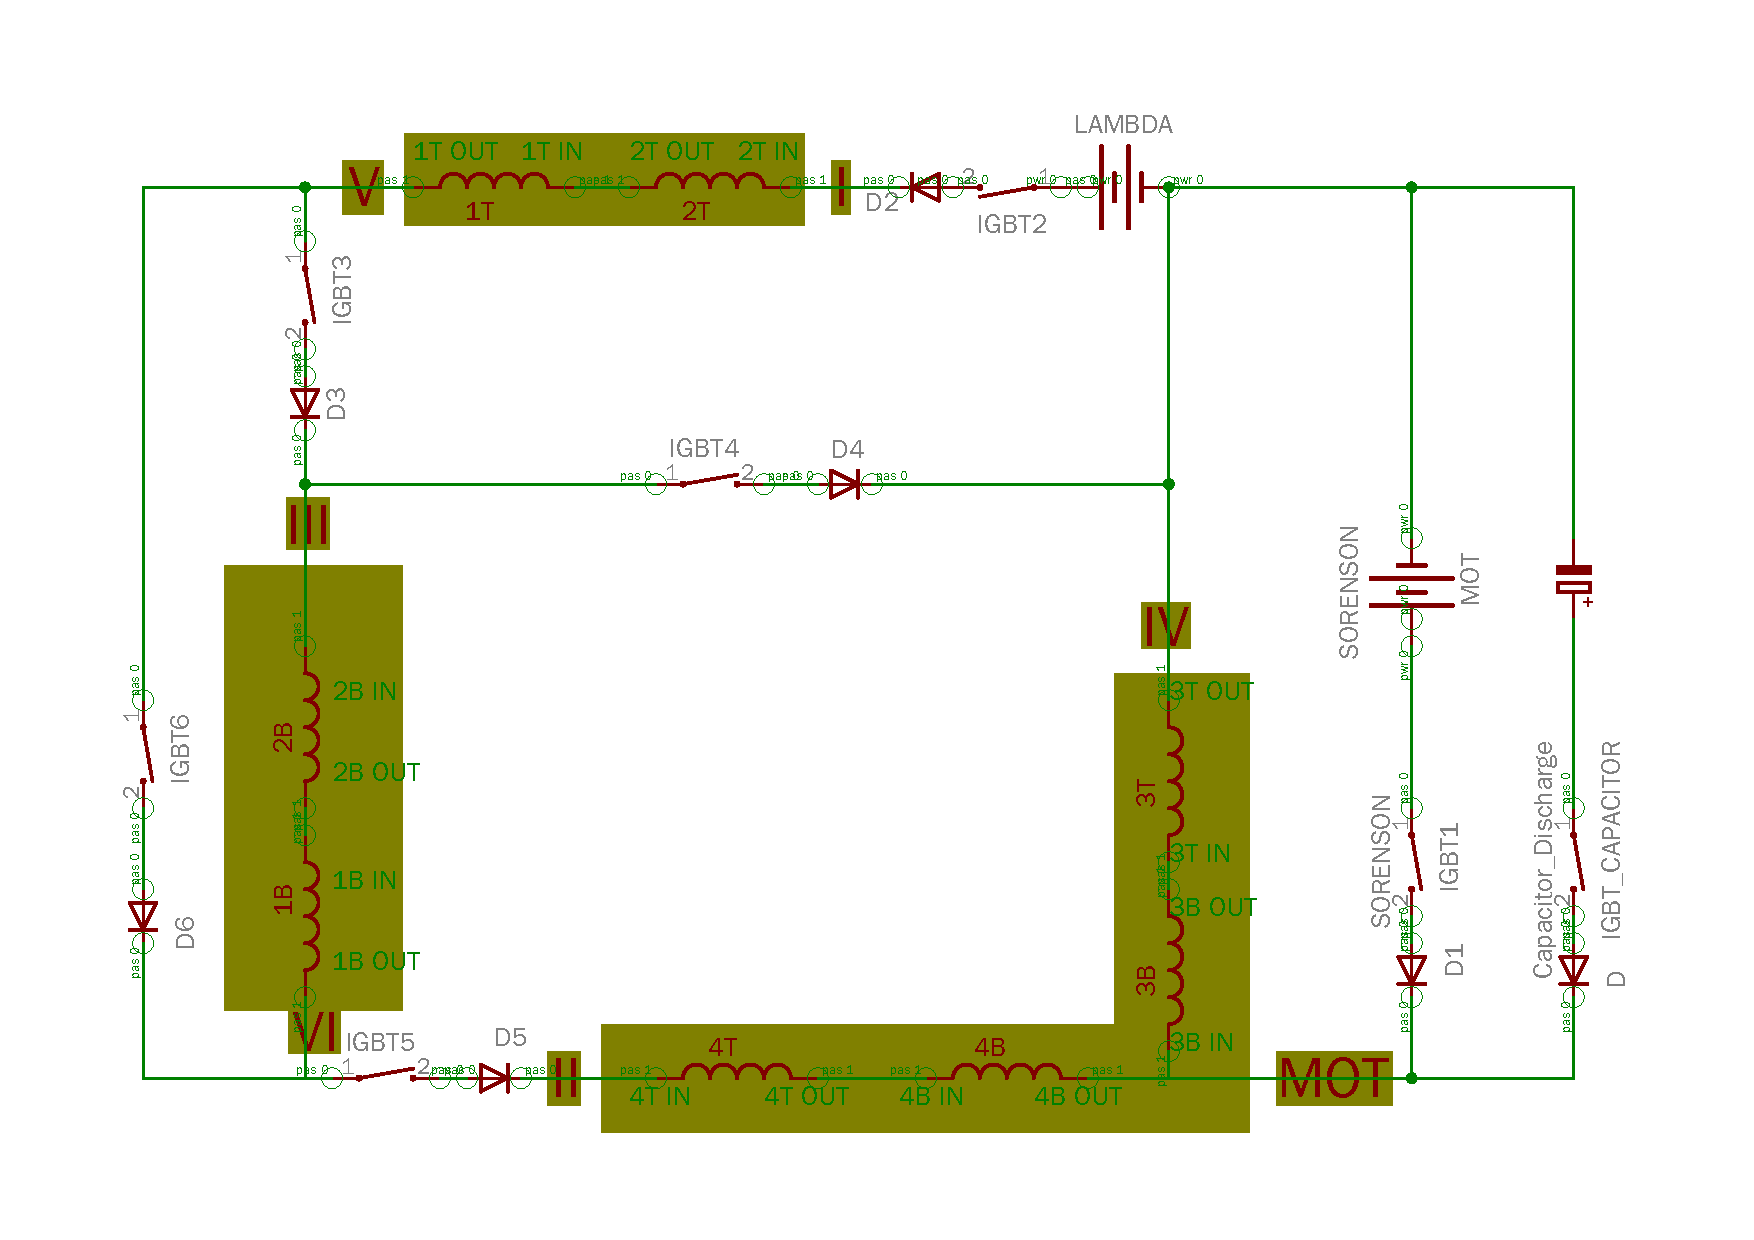
\includegraphics[width=12cm]{BEC5_coils.pdf}
  \end{center}
  \caption{Main Coils Control Circuit}
  \label{exp:coil-control}
\end{figure}
\begin{table}
  \begin{center}
    \begin{tabular}{|c|c|c|}\hline
      \multirow{2}{*}{Closed switches(IGBTs)}& \multicolumn{2}{c|}{Usage of the power supply} \\\hhline{~--}
      &Lambda&Sorenson\\\hline
      1, 3, 5&-&\begin{tabular}{@{}c@{}}Quadrupole field with\\layer 3 for MOT and ODT\\clean up (\ref{exp:odt})\end{tabular}\\\hline
      2, 3, 5&\begin{tabular}{@{}c@{}}Quadrupole field with\\layer 1, 2, 3 and 4 for\\magnetic trap\end{tabular}&-\\\hline
      1, 2, 4, 6&\begin{tabular}{@{}c@{}}Homogeneous Feshbach resonance\\field with layer 1 and 2\end{tabular}&\begin{tabular}{@{}c@{}}Field gradient on top of\\the bias field with layer 3\\for tilt and levitation.\end{tabular}\\\hline
    \end{tabular}
  \end{center}
  \caption{List of coil configurations}
  \label{exp:coil-config}
\end{table}

\section{Magneto-Optical Trap (MOT) and Compressed-MOT}\label{exp:mot}

The MOT loading is optimized by changing the parameters of the lasers to maximize the number of atoms in the MOT after $6$ seconds of loading. The optimum settings we have found are listed in table \ref{exp:mot-param} and the performance of our MOT can be found in table \ref{exp:laser-cooling}.\\
\begin{table}
  \begin{center}
    \begin{tabular}{|c|c|c|c|c|}\hline
      MOT power&Repumper power&MOT detuning&Repumper detuning&MOT Current\\\hline
      $16$mW&$7$mW&$-38.5$mW&$-28$mW&$57$A\\\hline
    \end{tabular}
  \end{center}
  \caption{MOT parameters}
  \label{exp:mot-param}
\end{table}\\
Since our MOT is mainly optimized for loading rate, it is not necessarily optimized for density and cooling. Therefore, we added a compress-MOT (CMOT) step after the MOT in order to increase the density and decrease the temperature. In the CMOT step, we ramp the MOT frequency closer to resonance in $4.5$ms and decrease the intensity of the repumper. As a result, the cloud is compressed by radiation pressure and pumped to the $F1$ state. The temperature of the cloud is also decreased because of the decrease in scattering. Figure \ref{exp:cmot-image} shows the F pumping effect in the CMOT and the performance of the CMOT is listed in table \ref{exp:laser-cooling}.
\begin{figure}
  \begin{center}
    \subfigure[CMOT imaged with $F2$ light without $F$ pumping.]{
      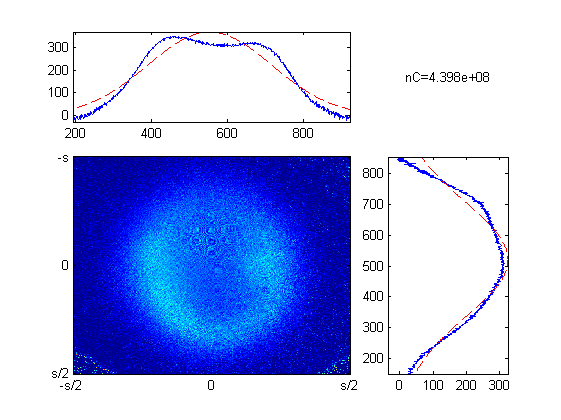
\includegraphics[width=5cm]{cmot-nopump.png}
    }
    \subfigure[CMOT imaged with $F2$ light after $F$ pump into $F2$.]{
      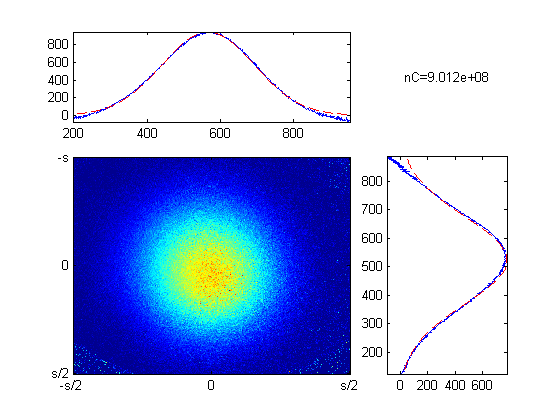
\includegraphics[width=5cm]{cmot-pump.png}
    }
  \end{center}
  \caption{Image of the CMOT. Atoms are pumped into the $F1$ states.}
  \label{exp:cmot-image}
\end{figure}

\section{Gray Molasses}\label{exp:gm}
The gray molasses step is used to cool the CMOT cloud further before transferring to the magnetic trap for evaporative cooling. Since the gray molasses beams have a smaller size ($d\approx5$mm), the beams need to be carefully aligned with the cloud which has a similar diameter. In our experiment, it is done putting F2 light in each gray molasses beam individually and imaging the overlap between the beam and the CMOT cloud directly. Figure \ref{exp:gm-align-nopump} shows the CMOT atoms after pumped into $F2$ state imaging with $F2$ light. After we pump the cloud with $F2$ light from one of the gray molasses beam path, the image looks like figure \ref{exp:gm-align-before}, in which the missing part is pumped back into $F1$ by the gray molasses beam and is invisible on the image. We then maximum the overlap between the beam and the cloud by minimize the atoms left in the image. Figure \ref{exp:gm-align-after} shows the same image after the gray molasses beam is properly aligned. After we repeated this on all the gray molasses beams, we took time of flight images while scanning the frequencies of the light. As shown in figure \ref{exp:gm-ddet}, a clear decrease in temperature (a decrease in time of flight size) can be seen just as what we expected from the theory\ref{theory:gm} and the experimental result from other groups\cite{gm-theory}.
\begin{figure}
  \begin{center}
    \subfigure[CMOT atoms pumped to $F2$]{
      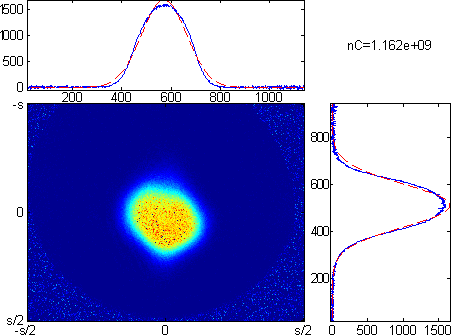
\includegraphics[width=6cm]{gm1-nopump.png}
      \label{exp:gm-align-nopump}
    }
    \subfigure[CMOT atoms pumped to $F2$ and hit with one of the gray molasses beam before alignment]{
      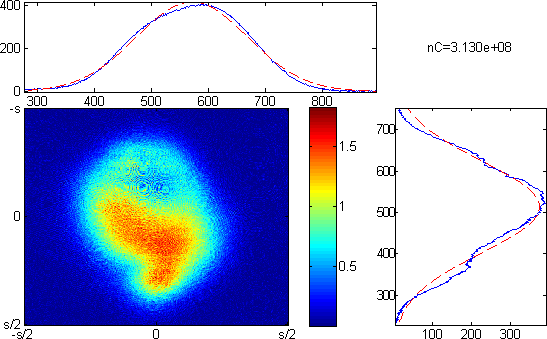
\includegraphics[width=6cm]{gm1-before.png}
      \label{exp:gm-align-before}
    }
    \subfigure[CMOT atoms pumped to $F2$ and hit with one of the gray molasses beam after alignment]{
      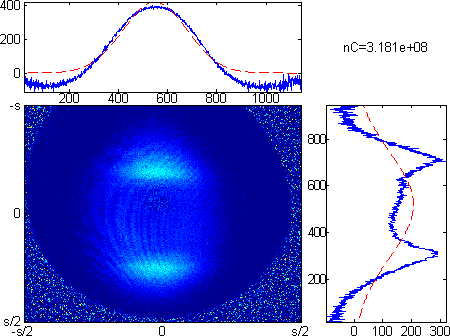
\includegraphics[width=4.5cm]{gm1-after.png}
      \label{exp:gm-align-after}
    }
  \end{center}
  \caption{Images used to align the gray molasses beams.}
  \label{exp:gm-align}
\end{figure}
\begin{figure}
  \begin{center}
    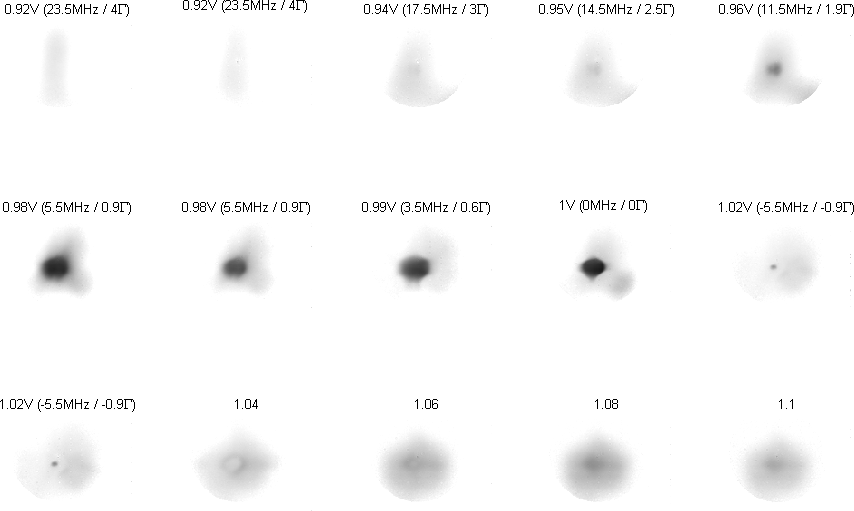
\includegraphics[width=11cm]{gm-ddet.png}
  \end{center}
  \caption{Time of flight image for gray molasses with different relative detuning (in MHz) between the pumper and repumper. (The voltages in the image is the control voltage we use to tweak the frequency.)}
  \label{exp:gm-ddet}
\end{figure}
\begin{table}
  \begin{center}
    \begin{tabular}{|c|c|c|c|c|}\hline
      Step&Atom Numbers&Temperature(K)&Density($\text{cm}^{-3}$)\\\hline
      Oven&-&$760$&-\\\hline
      Zeeman Slower&-&$0.5$&-\\\hline
      MOT&$2\cdot10^{10}$&$1.5\cdot10^{-3}$&$1\cdot10^{11}$\\\hline
      CMOT&$2\cdot10^{10}$&$1\cdot10^{-3}$&$2\cdot10^{11}$\\\hline
      Gray Molasses&$1\cdot10^{10}$&$1\cdot10^{-4}$&$2\cdot10^{11}$\\\hline
    \end{tabular}
  \end{center}
  \caption{Laser cooling performance.}
  \label{exp:laser-cooling}
\end{table}

\section{Dark State Pumping}\label{exp:pump}

At the end of Laser cooling, the atoms are distributed in different hyperfine levels not all of which are trappable. In order to transfer to and evaporate in the magnetic trap, all the atoms have to be in a single trappable state. Making use of the dark state in the $D1$ line with $\sigma^+$ light, we use the dark state pumping to transfer the atoms into the $|2, 2\rangle$ state without significant heating. In order to minimize re-scattering of the pumping light, the pumping light is blue detuned by $\delta_{F1}=20\text{MHz}$ and $\delta_{F2}=34\text{MHz}$. Figure \ref{exp:mf-pump-time} shows the atoms after different pumping time imaged with $D1F2$ $\sigma^+$ light. The initial increase in atom number shows atoms being pumped into $F2$ and the slower decay is when they are going into the $|2, 2\rangle$ state invisible to the imaging light.
\begin{figure}
  \begin{center}
    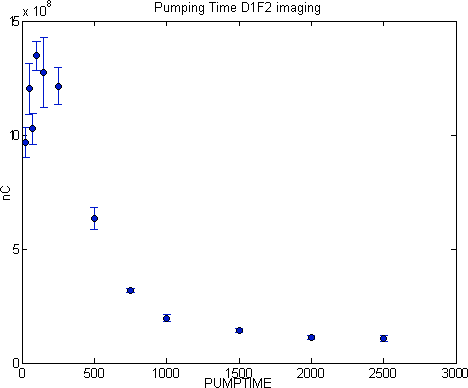
\includegraphics[width=8cm]{mf-pump.png}
  \end{center}
  \caption{}
  \label{exp:mf-pump-time}
\end{figure}

\section{Magnetic Trap}\label{exp:mt}
When the atoms are in the magnetic trap, the center of the trap need to be plugged in order to avoid Majorana loss. This is done with a $10$W $532$nm green laser beam, focused to $20\mu m$ at the center of the trap. In order to keep it aligned for different trap gradient, we zero the transverse magnetic field by measuring the center position of a small cloud in the magnetic trap with different gradients and different bias field. Figure \ref{exp:field-zeroing} shows the result of this measurement. We pick the bias field with the smallest displacement at different gradient, for which the center of the trap moves by smaller than one pixel ($20\mu m$). Figure \ref{exp:plug-power} shows the number of atom after the magnetic trap, the saturation of the atom number with $6$W of plug power shows that we have successful suppressed the Majorana loss. Due to the high inelastic collision rate, low elastic collision rate of Lithium-$7$ and the atom number fluctuation in our experiment, it is hard to optimize the RF evaporation purely experimentally. Instead, the evaporation in our experiment is optimized using numeric simulation. After $2.5$s of RF evaporation, we are left with $6\cdot10^7$ atoms with a temperature of $4\mu$K and a density of $10^{12}\text{cm}^{-3}$.
\begin{figure}
  \begin{center}
    \subfigure[$x$ direction]{
      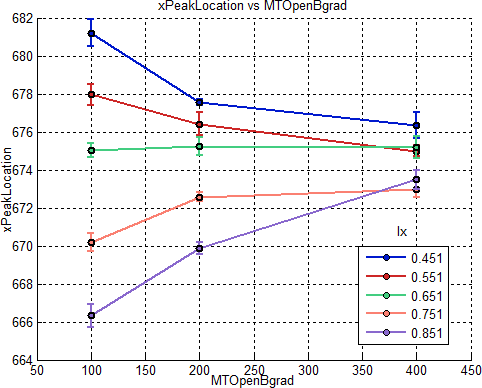
\includegraphics[width=5cm]{field-zeroing-x.png}
    }
    \subfigure[$y$ direction]{
      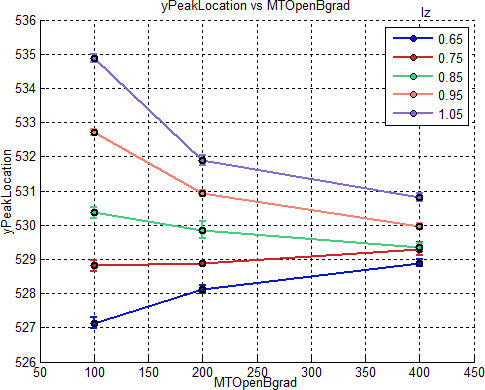
\includegraphics[width=5cm]{field-zeroing-y.png}
    }
  \end{center}
  \caption{Precise Field Zeroing in Magnetic trap}
  \label{exp:field-zeroing}
\end{figure}
\begin{figure}
  \begin{center}
    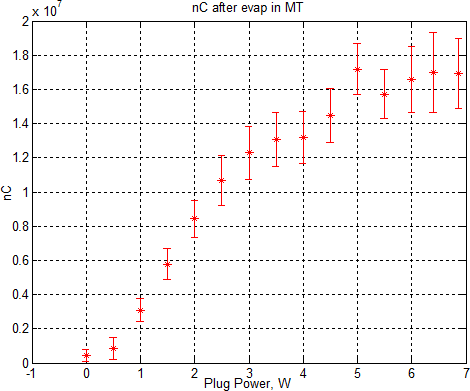
\includegraphics[width=9cm]{plug-power.png}
  \end{center}
  \caption{Saturation of the Plug Laser Power.}
  \label{exp:plug-power}
\end{figure}

\section{BEC in Optical Dipole Trap}\label{exp:odt}

After evaporation in the magnetic trap, we transfer the atoms into a optical dipole trap (ODT) created with two $15$W $1064$nm laser beams. The transfer need to be adiabatic in order to minimize heating and maximize transfer efficiency. After exploring different transfer schemes, the best method we have found is to turn on the ODT in full power before evaporating in the magnetic trap and ramp down the magnetic trap after evaporation in $200$ms. In this way, we can accumulate $2\cdot10^7$ atoms in the ODT at a temperature of $20\mu K$.\\
\\
We put the atoms from $|2, 2\rangle$ state to $|1, 1\rangle$ state using a Landau-Zener sweep with RF frequency. Figure \ref{exp:landao-zener} shows the atom number in $|2, 2\rangle$ versus starting frequency of a $1$MHz wide RF scan in a magnetic field about $1$G. We hit the resonance at $806.25$MHz and the transfer efficiency is better than $80\%$.\\
\begin{figure}
  \begin{center}
    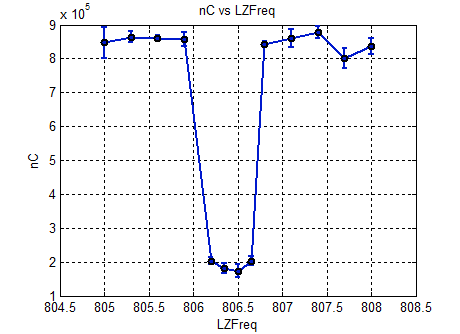
\includegraphics[width=9cm]{landao-zener.png}
  \end{center}
  \caption{Landau-Zener Sweep.}
  \label{exp:landao-zener}
\end{figure}\\
The evaporation in the ODT is aided by a Feshbach resonance. We measure the resonance using the increase in three-body loss rate. Figure \ref{exp:feshbach} shows the atom number after a certain hold time in the ODT with different Feshbach field. The resonance occurs at $285$A. By comparing the resonance point with know data for the scattering length around the resonance, we do our evaporation using a Feshbach current of $\approx275$A corresponding to a reasonably large scattering length ($\approx100a_0$).
\begin{figure}
  \begin{center}
    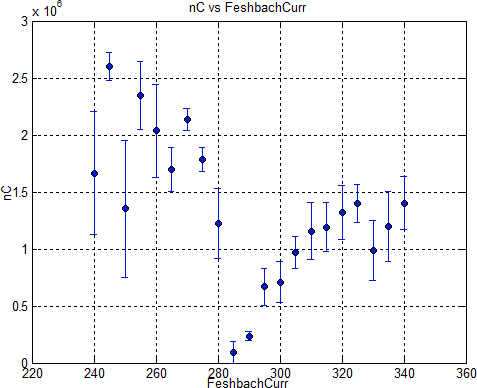
\includegraphics[width=9cm]{feshbach.png}
  \end{center}
  \caption{Feshbach Resonance in $|1, 1\rangle$ state.}
  \label{exp:feshbach}
\end{figure}

\begin{figure}
  \begin{center}
    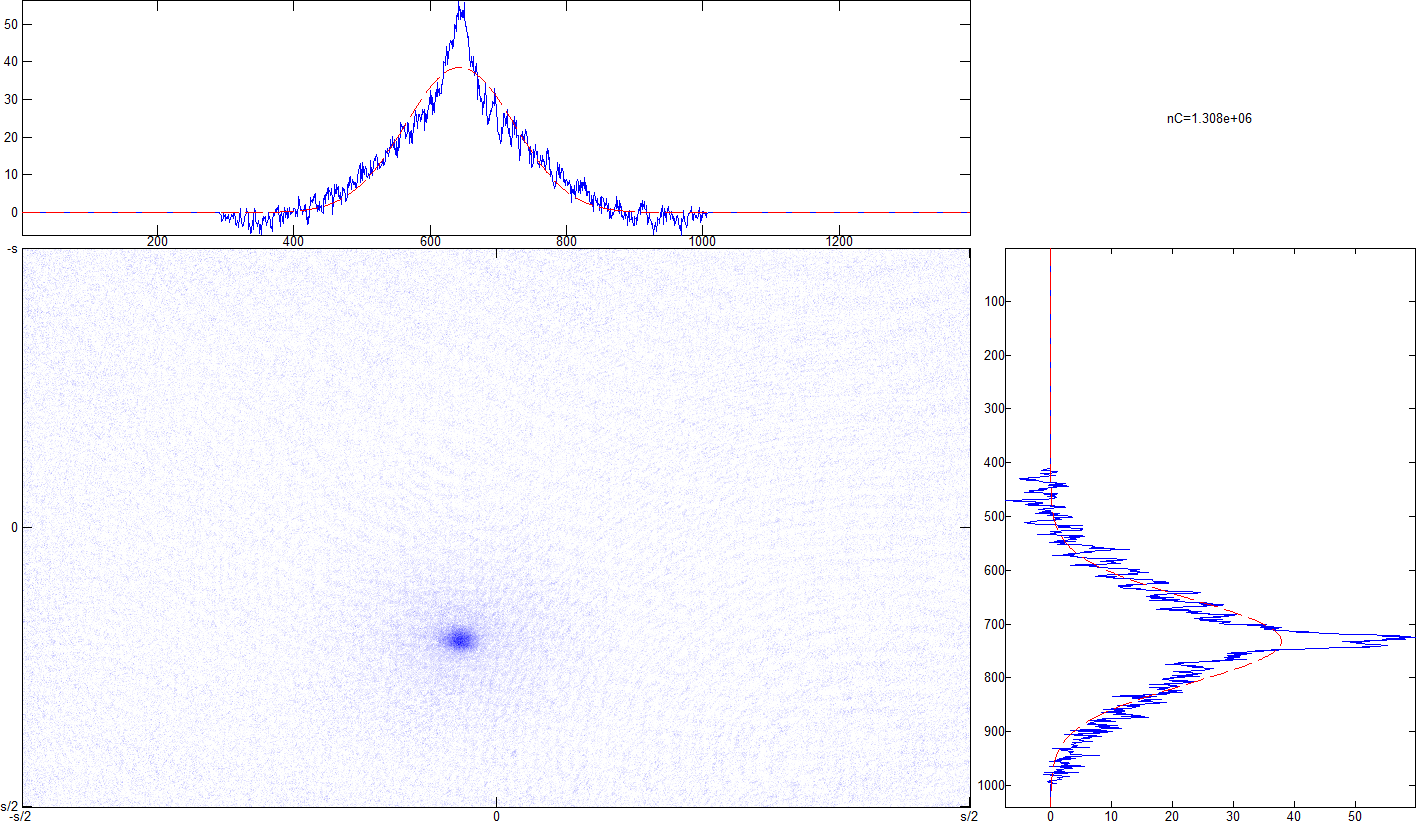
\includegraphics[width=9cm]{bec.png}
  \end{center}
  \caption{BEC with thermal wing.}
  \label{exp:bec-image}
\end{figure}
